\chapter{Background}
\label{chap:background}

\section{Compartmental Models for the Spread of Infectious Disease}
\label{sec:outbreak_models}

Compartmental epidemic models are used to describe the dynamics of an outbreak, to estimate how features of the population or environment affect its severity, and to understand how interventions might help to disrupt transmission. A compartmental model represents the time--evolution of an outbreak in terms of the disease histories of individuals as they transition between discrete states, or model compartments. When we use a compartmental model to describe the \textit{transmission} dynamics of an outbreak, the model compartments encode structural information about how individuals at different infection states interact to transmit the infectious agent. In contrast, states in a compartmental model for \textit{disease} dynamics typically correspond to discrete stages in the natural history of within--host disease progression without reference to the host's transmissive potential. This distinction is diagrammed in Figure \ref{fig:infec_vs_disease}.

Mechanistic compartmental models prescribe physical laws that govern the transmission dynamics of an outbreak. For example, the model might specify the rates of infectious contact between groups of people, or with an environmental reservoir that is a vector for transmission. Infection incidence and prevalence data are modeled conditionally on the mechanistic structure of the model, which specifies a functional form for the temporal and spatial evolution of the epidemic process. In contrast with their mechanistic counterparts, phenomenological models describe the data generating mechanism without explicit reference to the physical system that is under observation \cite{chowell2017fitting}. The price we pay for adopting a mechanistic approach is that our models will be obviously ``wrong", at least in the sense that all models are wrong, so it will be our responsibility to justifying their reasonableness. Our reward is that mechanistic models provide us with interpretable, multifaceted descriptions of outbreak dynamics. Moreover, the ubiquity of mechanistic models in the epidemiological literature enables us to incorporate information about specific aspects of transmission dynamics from other studies and settings into our own models. Historical overviews of mechanistic models for disease transmission may be found in \cite{anderson1992infectious,brauer2017mathematical,keeling2008,lessler2016mechanistic}.

Mechanistic compartmental models can be specified at varying levels of fidelity to the underlying epidemic process. Our models will range in granularity, from agent--based models in which we explicitly track the disease histories of individuals, to population--level models defined by the aggregate flow of individuals between model compartments. All of the models in this work will treat the epidemic process as evolving continuously in time, but observed at discrete times. The decision to work with continuous--time models is advantageous when observation times are not evenly spaced, or when various sub--processes evolve on different time scales \cite{glass2003,shelton2014}. Discrete--time models can be problematic when the epidemic and observation processes are misaligned, and do not necessarily produce results that are independent of the choice time--step (see \cite{shelton2014} for examples). One (very) compelling reason to prefer discrete--time models is that the computational effort required to fit them is typically much lower than what is required in the continuous--time setting. 

\subsection{An Agent--Based Susceptible--Infected--Recovered Model}
\label{subsec:sir_individual_mod}
For clarity of exposition, we will present the technical background on epidemic models in terms of the susceptible--infected--recovered (SIR model). Formal treatments that deal with this material in greater generality can be found in \cite{andersson2000stochastic,britton2018,brauer2008compartmental,fuchs2013inference,wilkinson2011stochastic}. The SIR model classifies individuals in a population of size $ N $ into one of three infection states: susceptible(S), infected (I), and recovered (R). Individuals are assumed to become infectious immediately upon entering the infected state, and acquire lasting immunity upon recovery. To simplify matters, we will assume the population is closed, meaning that there are no demographic changes or immigration, and that individuals are exchangeable. This latter assumption implies that individuals mix homogeneously and are alike in their infection dynamics. 

The SIR model defines an epidemic process, $ \bX = \lbrace\bX_1,\dots,\bX_N\rbrace $, that collects the subject--level subprocesses, $ \bX_j,\ j=1,\dots,N $, each of which takes values in the state space of disease state labels, $ \mcS_j= \lbrace S,I,R\rbrace $. A realized subject--path is of the form 
\begin{equation}
\bx_j = \left \lbrace\begin{array}{ll}
S,\ & \tau < \tau_I^{(j)},\\
I,\ & \tau_I^{(j)}\leq\tau<\tau_R^{(j)},\\
R,\ & \tau_R^{(j)} \leq \tau,
\end{array}\right .
\end{equation}
where $ \tau_I^{(j)} $ and $ \tau_{R}^{(j)} $ are the infection and recovery times for subject $ j $, and are possibly infinite (Figure \ref{fig:subjectsamplepaths}). The state space of $ \bX $ is  $ \mcS = \lbrace S,I,R\rbrace^N $, the Cartesian product of subject--level state labels. We denote by $ \bX(\tau) = \left (\bX_1(\tau),\dots,\bX_N(\tau)\right ) $ the state of $ \bX $ at time $ \tau $, and by $ \bX(\tau^+) $ the state just after time $ \tau $. 

\begin{figure}[htbp]
	\centering
	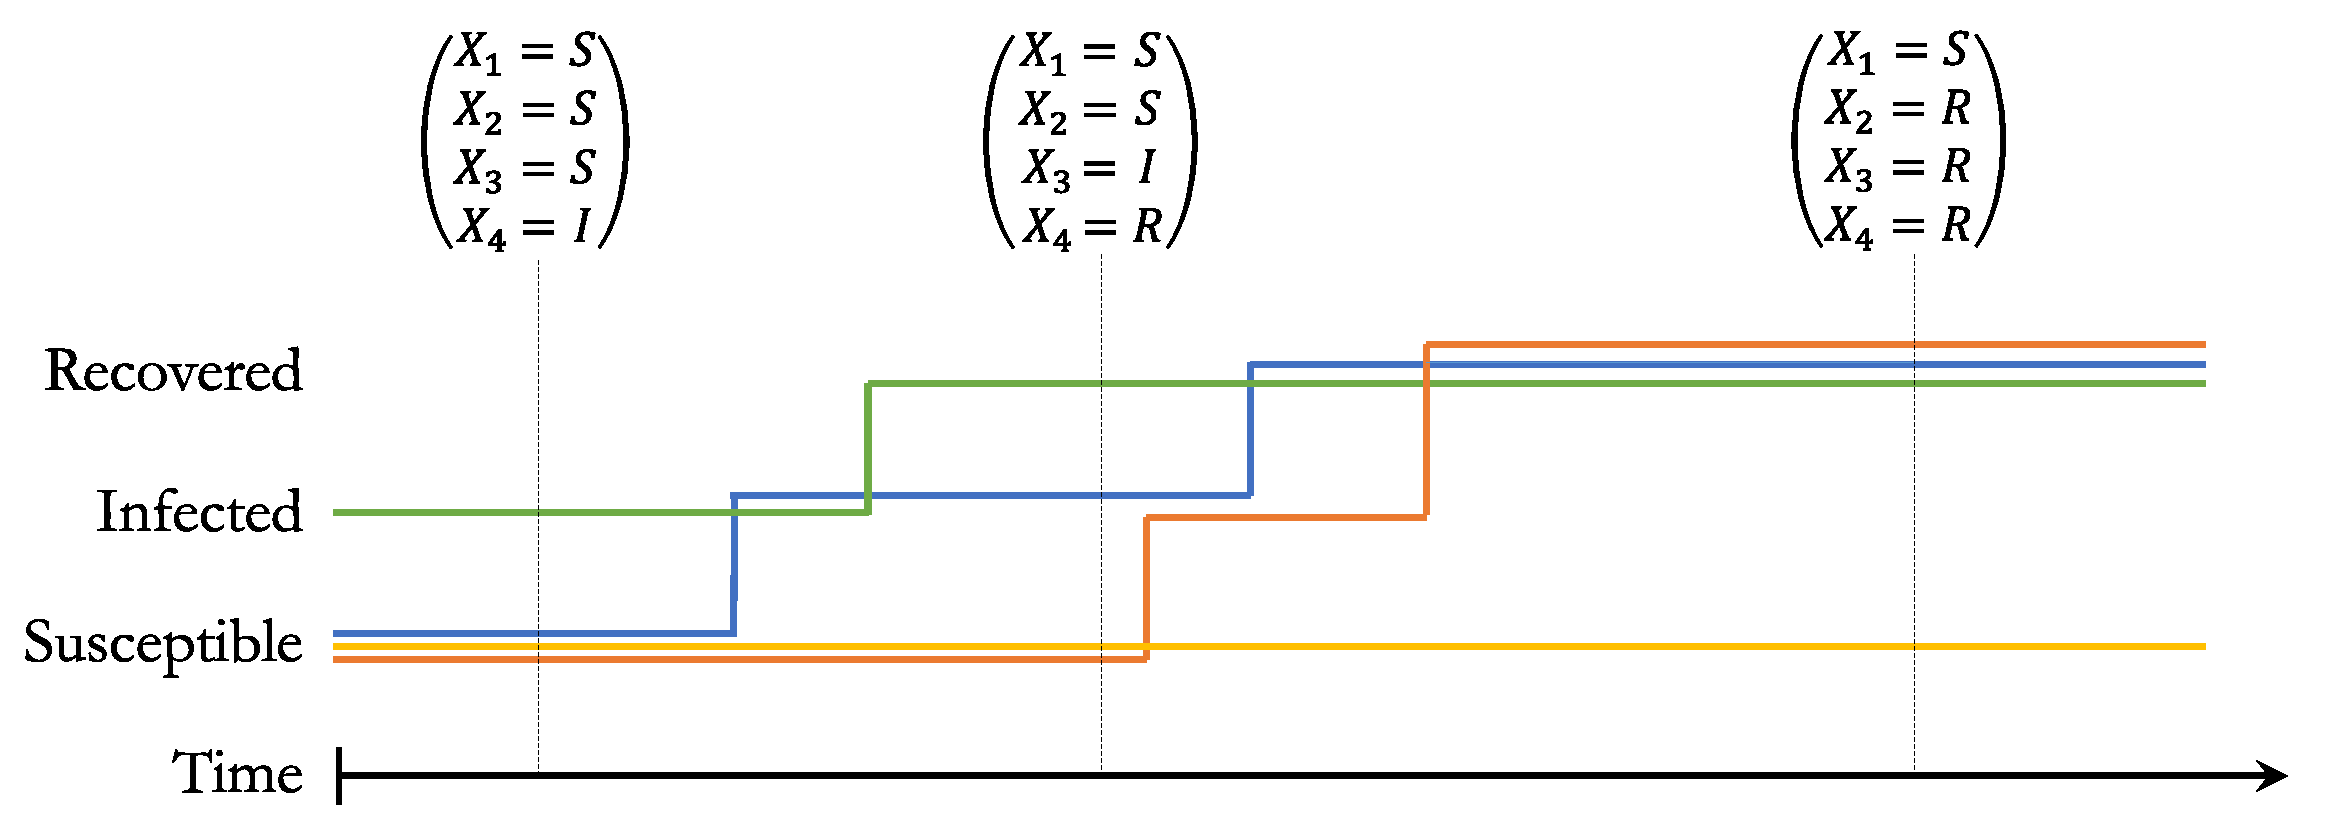
\includegraphics[width=0.8\linewidth]{figures/subject_sample_paths}
	\caption{Diagram of subject--level paths (colored lines) for an SIR model in a population of size $ N=4 $. Individuals transition through infection states continuously in time. The epidemic process is defined in terms of the infection states of individuals in the population.}
	\label{fig:subjectsamplepaths}
\end{figure}

The waiting times between subject--level transition events are typically taken to be exponentially distributed. This will allow us to take advantage of several useful properties of exponential random variables (Figure \ref{fig:exp_props}, see \cite{wilkinson2011stochastic} for proofs). Critically, this choice also implies that $ \bX $ evolves as a continuous--time Markov chain (CTMC) with transition rate from configuration $ \bX $ to $ \bX^\prime $, differing only in the state of a single subject, given by
\begin{equation}
\lambda_{\bX,\bX^\prime} = \left \lbrace \begin{array}{rl}
\beta I,\ &\text{if } \bX\ \text{and } \bX^\prime\ \text{differ only in subject }j \text{, with }\bX_j=S\text{, and }\bX_j^\prime=I,\\
\mu,\ &\text{if } \bX\ \text{and } \bX^\prime\ \text{differ only in subject }j \text{, with }\bX_j=I\text{, and }\bX_j^\prime=R,\\
0,\ & \text{for all other configurations }\bX\ \text{and }\bX^\prime.
\end{array}\right.
\end{equation}
with per--contact infection rate,  $ \beta $, and recovery rate, $ \mu $. That $ \bX $ is a \textit{Markov} process means that its forward--time evolution depends on its history only through its current state, i.e.,
\begin{equation}
\label{eqn:sir_markov}
\Pr\left (\bX(\tau + \dtau) = \bx | \lbrace\bX(\tau) = \bx(\tau),\ \tau\in[0,\tau]\rbrace, \btheta\right ) = \Pr\left (\bX(\tau + \dtau) = \bx | \bX(\tau) = \bx(\tau),\btheta\right ).
\end{equation}
$ \bX $ is \textit{time--homogeneous} since the rates of transition between configurations in the state space of $ \bX $ are constant over time. In contrast, the subject--level subprocess, $ \bX_j $, is a \textit{time--inhomogeneous} CTMC with transition rate matrix
\begin{equation} 
\label{eqn:sir_subj_rate_mtx}
\bLambda^{j}(\btheta)(\tau) = \bordermatrix{ & S & I & R \cr
	S & -\beta I^{(-j)}(\tau) & \beta I^{(-j)}(\tau) & 0 \cr 
	I & 0 & -\mu & \mu \cr
	R & 0 & 0 & 0 },
\end{equation}
 since $ I^{(-j)}(\tau) $, the number of infected individuals in the population at time $ \tau $, excluding individual $ j $, changes over time. 

\begin{figure}[htbp]
	\caption{Very useful properties of exponential random variables.}
	\label{fig:exp_props}
	\begin{itemize}
		\item (Memoryless property) If $ Z\sim\mr{Exp}(\lambda)$, then $ \forall t,\dt\geq0 $  we have \begin{equation}
		 \Pr(Z > t+\dt | Z>t) = \Pr(Z>\dt).
		\end{equation}
		\item (Racing exponentials) If $ Z_i\sim\mr{Exp}(\lambda_i),\ i=1,\dots,n $, are independent, then \begin{equation}
		\underset{i}{\mr{min}}(Z_i) \sim \mr{Exp}\left (\lambda = \sum_i\lambda_i\right ).
		\end{equation}
		\item (Index of minimum) If $ Z_i\sim\mr{Exp}(\lambda_i),\ i=1,\dots,n $, are independent, then the index $ k $ of the minimum of $ Z_i $ is a random variable with probability mass function \begin{equation}
		\Pr(k|Z_k = \min(Z_1,\dots,Z_n)) = \frac{\lambda_k}{\sum_j\lambda_j}.
		\end{equation} 
	\end{itemize}
\end{figure}

Let $ \btau = \lbrace\tau_0,\dots,\tau_{K+1}\rbrace $, be the (ordered) set of $ K $ infection and recovery times of all individuals along with the endpoints of the time period $ [\tau_0,\ \tau_{K+1}] $. Let $ \ind{\tau_k \corresponds I} $ and $ \ind{\tau_k \corresponds R} $ indicate whether $ \tau_k $ is an infection or recovery time, and let $ \btheta = (\beta, \mu, \bX_0) $ denote the vector of parameters, including the initial state of $ \bX $ at time $ \tau_0 $. The CTMC likelihood of $ \bX $ over $ [\tau_0,\ \tau_{K+1}] $ is a product of exponential waiting time densities,
\begin{align} 
\label{eqn:sir_subj_likelihood}
L(\bX| \btheta) &= \prod_{k = 1}^{K}\left \lbrace \left [\beta I_{\tau_k}\times\ind{\tau_k \corresponds I} + \mu\times\ind{\tau_k \corresponds R}\right ] \exp{\left [-\left (\tau_k - \tau_{k-1}\right )\left (\beta I_{\tau_k} S_{\tau_k} + \mu I_{\tau_k}\right )\right ]}\right \rbrace \nonumber \\
& \hspace{0.2in} \times \exp \left [-\left (t_L - \tau_K\right )\left (\beta I_{\tau_K^+}S_{\tau_K^+} + \mu I_{\tau_K^+}\right )\right ]. 
\end{align}

\subsection{A Population--Level Susceptible--Infected--Recovered Model}
\label{subsec:sir_population_mod}
The subject--level SIR model is exactly equivalent to the population--level SIR model that is often preferred for various computational reasons \cite{andersson2000stochastic,allen2008introduction}. This equivalence derives from a property of Markov processes called \textit{lumpability} \cite{tian2006lumpability}. 

Given a Markov process, $ \bX $ with state space $ \mcS = \lbrace s_1,\dots,s_P\rbrace $ and initial probability vector $ \pi $, we define a new process, $ \overline{\bX} $ on state space $ \overline{\mcS} = \lbrace S_1,\dots,S_\mathcal{L}\rbrace $, a partition of $ \mcS $. The jump chain of this new chain is obtained by taking the sequence of subsets of $ \overline{\mcS} $ that contain the corresponding states of the original jump chain. The initial probability distribution of $ \overline{\bX}(t) $ is \begin{equation*}
\Pr(\overline{\bX}(t_0) = S_i) = \mathrm{Pr}_\pi(\bX(t_0) \in S_i)
\end{equation*}
and its transition probabilities are given by
\begin{equation*}
\Pr(\overline{\bX}(t+\Delta t) = S_j | \overline{\bX}(t)=\overline{\bx}(t^\prime), t^\prime \leq t) = \Pr(\overline{\bX}(t+\Delta t) \in S_j | \bX(t)=\bx(t^\prime), t^\prime \leq t),
\end{equation*}
where $ \overline{\bx}(t^\prime) $  and $ \bx(t^\prime) $ denote the paths of the original process and the new process. The new process is called the \textit{lumped process}. We say that the original process is \textit{lumpable} with respect to a partition $ \overline{\mcS} $ of $ \mcS $, and that $ \overline{\bX}(t) $ is the \textit{lumped Markov process} corresponding to $ \bX(t) $, if for every choice of $ \pi $ we have that $ \overline{\bX}(t) $ is Markov and the transition probabilities do not depend on $ \pi $. A necessary and sufficient condition for a CTMC to be lumpable is that its rate matrix, $ \bLambda = (\lambda_{a,b}) $, where $ \lambda_{a,b} $ being the rate of transition from $ s_a $ to $ s_b $, satisfies
\begin{equation*}
\sum_{s_b \in S_B}\lambda_{a,b} = \sum_{s_b \in S_B}\lambda_{c,b}
\end{equation*}
for any pair of sets $S_A$ and $ S_B$ and for any pair of states  $(s_a, s_c)$  in $S_A \in \overline{\mcS} $. 

\begin{figure}
	\centering
	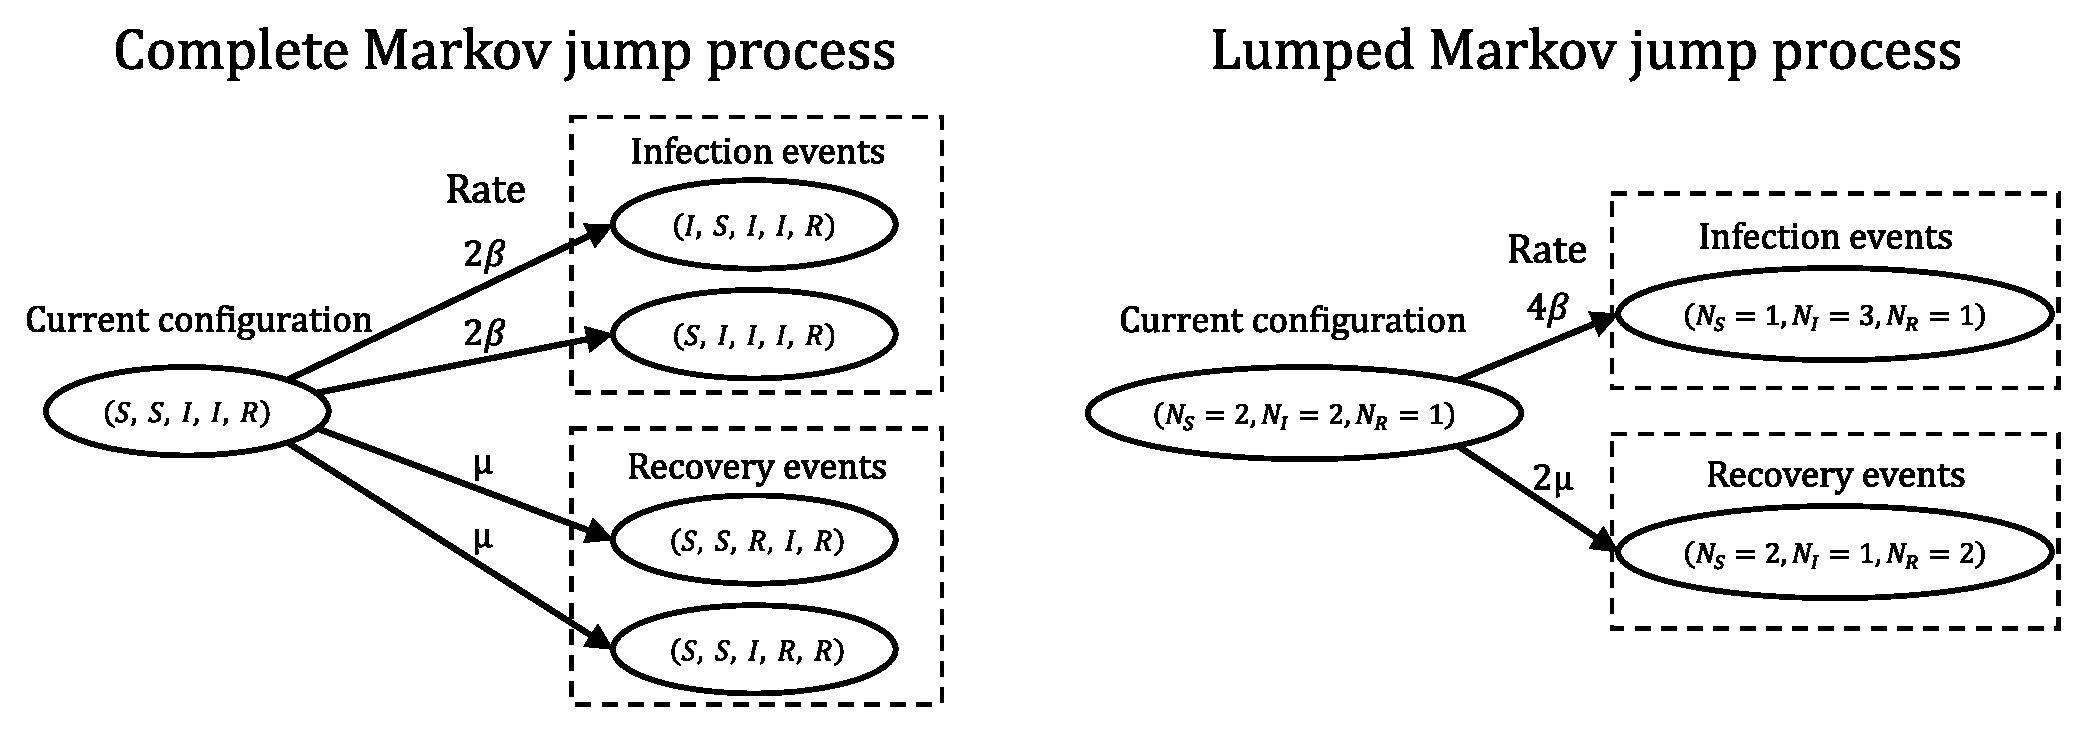
\includegraphics[width=0.9\linewidth]{figures/SIR_representations}
	\caption{Complete and lumped representations of SIR dynamics in a population of five individuals. The per--contact infectivity rate, $ \beta $, and the recovery rate, $ \mu $, parameterize exponential waiting time distributions between transition events. The complete Markov jump process evolves on the state space of subject state labels, $ \mcS = \lbrace S,I,R\rbrace^N $, with dynamics determined by the subject--level transition rates. Each susceptible may contact two infected individuals, while each infected individual recovers independently. The lumped process evolves on the state space of compartment counts, $ \widebar{\mcS} = \lbrace N_S,N_I,N_R:\ N_S + N_I+N_R=N\rbrace $, with dynamics determined by lumped transition rates. The waiting time distributions between transitions are derived by noting that if $ \tau_1\sim \exp(\lambda_1) $ and $ \tau_2\sim\exp(\lambda_2) $, then $ \tau_{\min} = \min(\tau_1,\tau_2)\sim\exp(\lambda_1+\lambda_2) $.}
	\label{fig:sirrepresentations}
\end{figure}

In Section \ref{sec:methods_sir}, we defined the latent process, $ \bX(\tau) = (\bX_1,\dots,\bX_N)$, with state space $ \mcS = \lbrace S, I, R\rbrace^N $. Let $ c_u = (x_1,\dots,x_N) $ denote a configuration of the state labels (e.g. $ c_u = (S, I, S, R, I) $), and denote the set of configurations that correspond to a vector of compartment counts by $$ \mcC_{lmn} = \left \lbrace c_u:l=\sum_{i=1}^N\ind{x_i = S},m=\sum_{i=1}^N\ind{x_i=I},n = \sum_{i=1}^N\ind{x_i=R},\ l+m+n=N \right \rbrace. $$ 
The state space of count vectors, 
$$ \overline{\mcS} = \left \lbrace \mcC_{lmn}: l,m,n \in \lbrace1,\dots,N\rbrace, l+m+n = N \right \rbrace, $$ 
defines a partition of $ \mcS $ that is obtained by stripping away the subject labels and summing the number of individuals in each disease state. 

Given the partition $ \overline{\mcS} $ of $ \mcS $, we may define the CTMC for the canonical SIR model, $ \overline{\bX} = (N_S, N_I, N_R) $, where $ N_S + N_I + N_R = N $ and $ N_S,N_I,N_R \in \lbrace0,\dots,N\rbrace $, on the state space of compartment counts, depicted in Figure \ref{fig:sirrepresentations}. This construction is usually presented for computational reasons since discarding the subject labels for infection and recovery events substantially reduces the computational overhead. When the sojourn times are exponentially distributed, the transition rates for the time-homogeneous CTMC are 
\begin{equation*}
\begin{array}{cc}
\underline{\text{Transition}} & \underline{\text{Rate}} \\
(N_S,N_I,N_R) \longrightarrow (N_S-1,N_I+1,N_R) & \beta N_S N_I ,\\
(N_S,N_I,N_R) \longrightarrow (N_S,N_I-1,N_R+1) & \mu N_I .
\end{array}
\end{equation*}

The state space $ \overline{\mathcal{S}} $ partitions the state space $ \mathcal{S} $ into groups of configurations for which the triple of compartment counts are the same. The CTMC $\overline{\bX}$ trivially satisfies the condition for lumpability, and thus is the lumped Markov chain of $ \bX $ with respect to this partition.

A Markov process is lumpable with respect to a partition of its state space if there exists another Markov process  A Markov process is \textit{commutative} with respect to a lumping of its state space if the lumped jump chain of the original process has the same distribution as the jump chain of the lumped process on the partitioned state space. We now explain these two very confusing sentences, but refer to \cite{tian2006lumpability} for a more thorough discussion. 

 

there is a lumped Markov process taking values 

with a state space that groups together, or lumps, elements of the original state space, and that is has jum

\subsection{A Dubiously Brief Review of CTMCs}
\label{subsec:ctmc_overview}
We interrupt our regularly scheduled broadcasting to 


\subsection{Deterministic Representations}
\label{subsec:deterministic_models}


\subsection{Large--Population Approximations}
\label{subsec:large_pop_approx}

\subsubsection{Diffusion approximations of Markov jump processes}
\label{subsubsec:diff_approx}

\subsubsection{Linear noise approximation}
\label{subsubsec:lna_background}

\section{Computational Approaches to Fitting Stochastic Epidemic Models}
\label{sec:computational_background}

\section{Bayesian Computation and Markov Chain Monte Carlo}
\label{sec:bayesian_computation}

\subsection{Markov Chain Monte Carlo}
\label{subsec:mcmc}

\subsubsection{Bayesian Data Augmentation}
\label{subsec:data_augmentation}

\subsubsection{Slice sampling}
\label{subsubsec:slice_sampling}

\subsubsection{Elliptical slice sampling}
\label{subsubsec:elliptical_slice_sampling}

\subsubsection{Adaptive multivariate normal slice sampling}
\label{subsubsec:mvn_slice_sampling}